\documentclass[25pt, portrait, a1paper]{tikzposter}
\usepackage{tikz}
\usepackage{adjustbox}
\usepackage{textcomp}
\usepackage{multicol}
\usepackage{amsmath}
% \usepackage{amssymb}
\usetikzlibrary{shapes, arrows.meta}
\usetheme{Default}

\begin{document}

%   \begin{columns}
%     \column{0.5}
  \block[titleoffsety=.49\textheight, bodyoffsety=.49\textheight, bodywidthscale=1.04, titlewidthscale=1.04]{More details on models and methods}{
	\innerblock{Construction of the PES}{
	  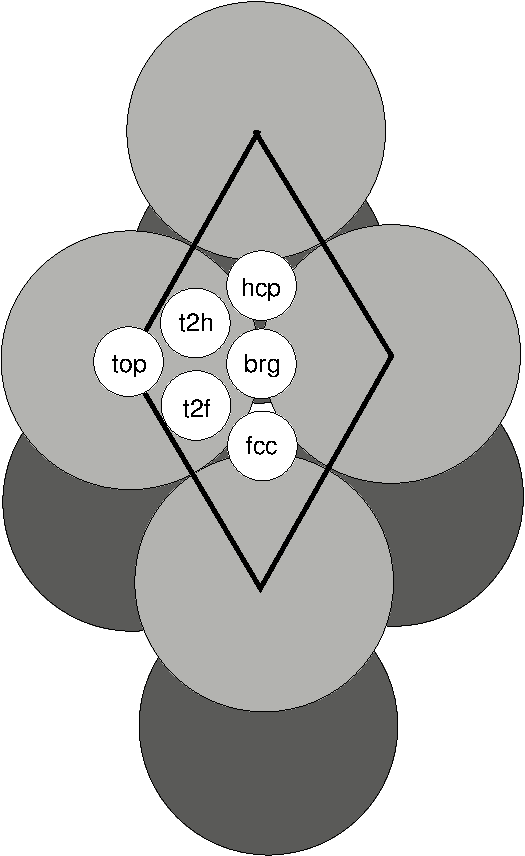
\includegraphics[width = .1\textwidth]{abb/fig_1a-eps-converted-to.pdf}
	}
	\vspace{\baselineskip}
	\innerblock{Details of the GLO}{
	  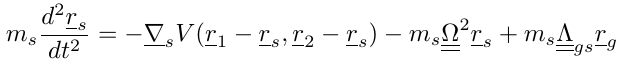
\includegraphics[width = .8\textwidth]{abb/GLO_eq1.png}
	  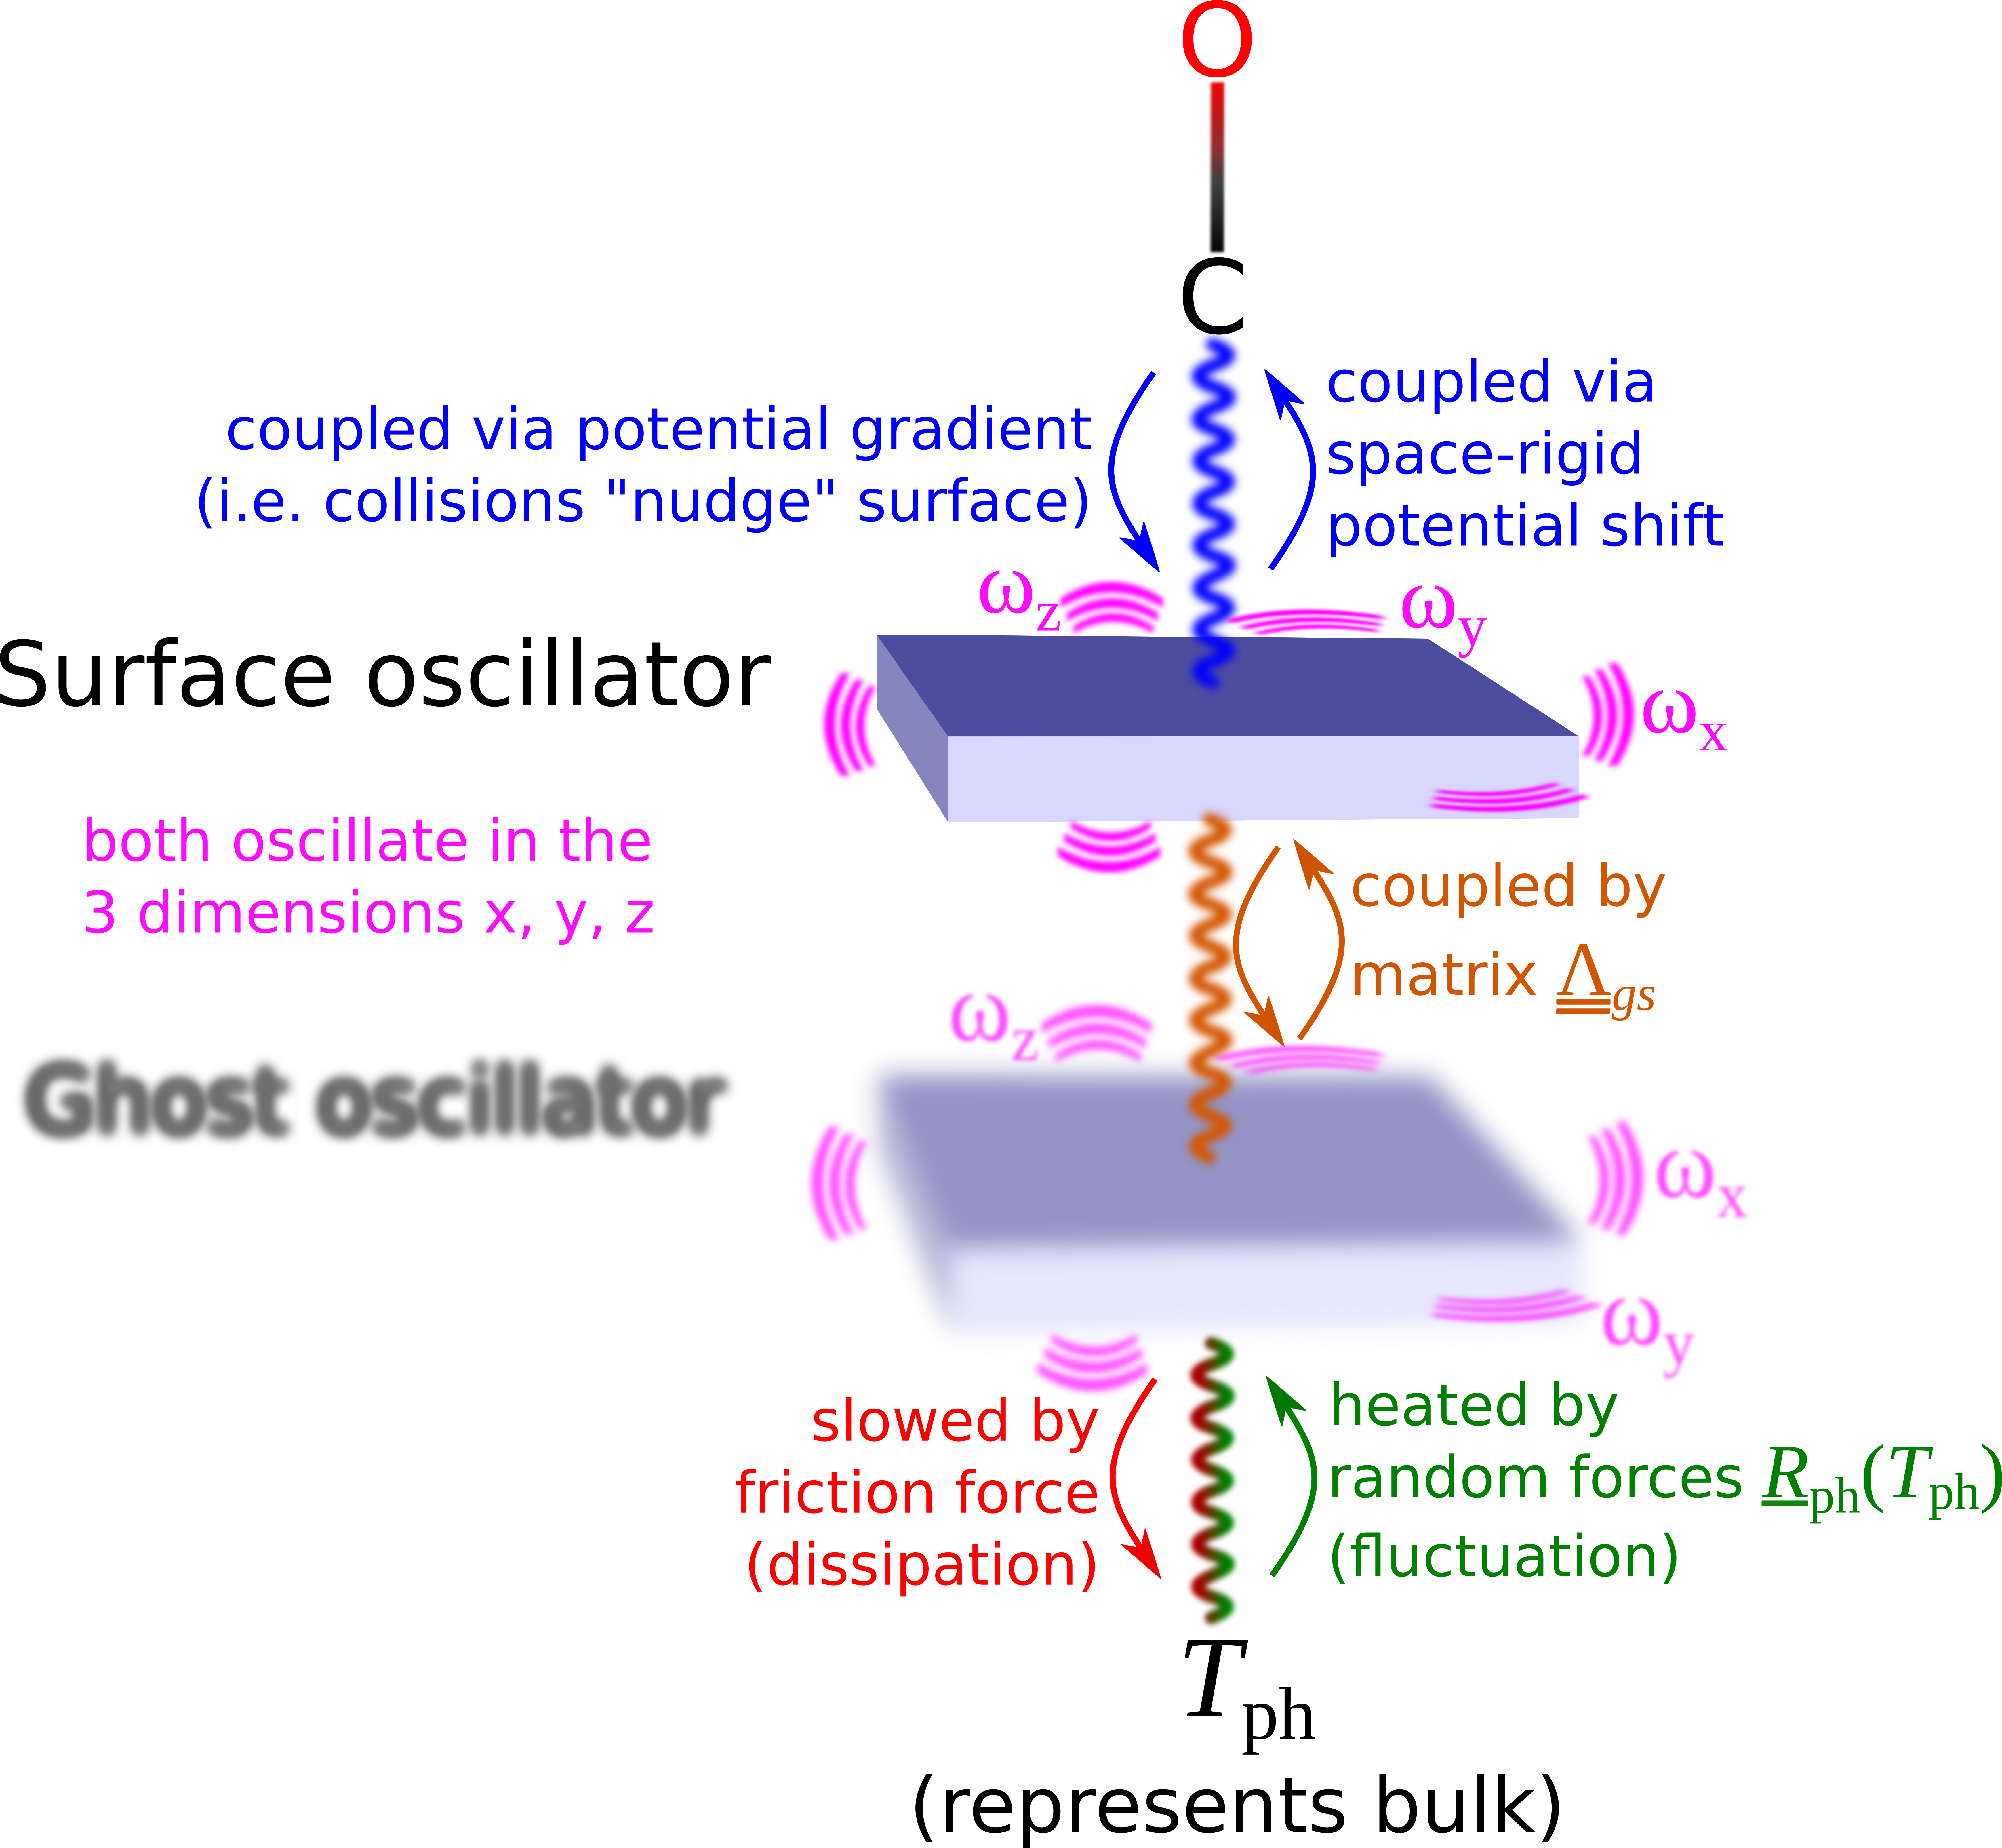
\includegraphics[width = .5\textwidth]{abb/GLO.png}
	}
	\vfill
  }
  \block[bodywidthscale=0.1]{}{}
  \note[width = 15cm]{\textbf{Contact information:}\\
	Robert Scholz\\
	Haus 25, Raum D2.04/05\\
	Institut f\"ur Chemie\\
	Universit\"at Potsdam\\
	Karl-Liebknecht-Str. 24-25\\
	D-14476 Potsdam\\

  
	\textbf{Email: robscholz87@hotmail.com}
  }
%     \column{0.5}    
%   \end{columns}
\end{document}
